% This is the section 'V2-0Abstract' to the "Hodgkin-Huxley neuron model V2.0 book"
% Last edited 2026.08.23

\ifx\magyar\undefined
\section[The abstract neuron]{The abstract neuron\label{sec:V2-0_AbstractNeuron}}

\else

\section[Az absztrakt neuron]{Az absztrakt neuron\label{sec:V2-0_AbstractNeuron}}
\fi


\ifx\magyar\undefined
Nature uses an infinite variety of implementing neurons. 
In the \gls{CNS} 
they can cooperate
with each other, 'despite the extraordinary diversity and complexity of neuronal morphology and synaptic connectivity,
\textit{the nervous systems adopt \textbf{a number of
 basic principles}} for all neurons and synapses',
\cite{JohnstonWuNeurophysiology:1995}
independently from the infinitely complex molecular, biochemical and physiological details.
Nature focuses only on functionality, the design of an element is irrelevant as long as the element performs its task. Malfunctions are of course tied to the specific implementation.
\index{Johnston Daniel}
\index{Wu Samuel Miao-sin }
We \textit{will base our holistic discussion on those general basic principles 
and create an 
\hyperlink{NeuronPhysical}
{'abstract physical neuron'}; a hypothetical element, which functions
essentially like a neuron},
skipping the 'implementation details' nature uses.
We essentially follow von Neumann's method in describing the foundations of
computing science~\cite{EDVACreport1945}: "we will base our considerations on a hypothetical element, which functions essentially like a neuron".
We need \hyperlink{Abstractions}
{different abstractions and approximations} 
(furthermore, \hyperlink{NonOrdinaryLaws}{'non-ordinary' laws} of science) for describing biological processes.
\index{ordinary laws}

However, an abstraction is usable
in practice only when paired with a generalization: the more abstract the assumption, the more general and widely applicable the concept or conclusion.
\textit{By abstractions, we can reduce the unbelievably detailed world into manageable pieces, and we can learn anything general.}
We must show which approximations are oversimplifications and which phenomena are misunderstood; measured, or interpreted in a wrong approach.

\else

A természet végtelenül változatos módokon valósít meg neuronokat.
A központi idegrendszerben (\gls{CNS}) ezek egymással együtt tudnak működni, mivel 'despite the extraordinary diversity and complexity of neuronal morphology and synaptic connectivity,
\textit{the nervous systems adopt \textbf{a number of
 basic principles}} for all neurons and synapses',
\cite{JohnstonWuNeurophysiology:1995}
azok rendkívül összetett molekuláris, biokémiai és fiziológiai 
részletei ellenére.
A természet csupán a funkcionalitásra koncentrál, egy-egy elem  kivitelezése mindaddig lényegtelen, amíg az elem ellátja a feladatát. A hibás működés természetesen a konkrét megvalósításhoz kötődik.
\index{Johnston Daniel}
\index{Wu Samuel Miao-sin}
Átfogó tárgyalásunkban ezekre az általános elvekre támaszkodunk
és egy \hyperlink{NeuronPhysical}
{'abstract physical neuron'}-nak nevezett hipotetikus elemet
hozunk létre, ami lényegében úgy működik, mint egy neuron;
átugorva az "implementációs részleteket".
Lényegében Neumann Jánosnak a számítástudomány alapelveit 
leíró munkájában~\cite{EDVACreport1945} vezetett be:
"we will base our considerations on a hypothetical element, which functions essentially like a neuron".

Különböző  \hyperlink{Abstractions}
{absztrakciók és közelítések},
(továbbá, \hyperlink{NonOrdinaryLaws}{a tudomány 'rendetlen' (non-ordinary) törvényeinek} ) felhasználásával  írjuk le a biológiai
folyamatokat.
\index{rendetlen törvények}
Azonban a gyakorlatban egy absztrakció csak akkor használható,
ha egy általánosítással párosítjuk. Minél absztraktabb egy feltevés,
annál szélesebb körben használható a fogalom vagy következtetés.
\textit{Az absztrakciók által a hihetetlenül gazdag világot
kezelhető darabokra bontjuk és általános dolgokat tanul\-hatunk.}
Meg kell mutatnunk hogy melyik közelítés túlegyszerűsítés
és milyen tapasztalatokat értettünk félre; mértünk vagy értelemeztünk rosszul.
\fi


\ifx\magyar\undefined
In our  science-based non-disciplinary model (the 'abstract physical neuron', as we call it), a neuron (highly simplified) is an elastic sphere with two lipid layers (membrane) in an electrolyte, a similarly elastic insulating output tube (axon), and an incompressible, partially ionized electrolyte fluid with different compositions and concentrations inside and outside.
In addition to ions, the electrolyte segments contain simple chemical molecules, and complex biological formations.
The electolytes inside and outside  may have gradients and the ions move at continuously changing speeds that can vary by several orders of magnitude during operation. 
The lipid layer is partially permeable (controlled or uncontrolled) for the components above (channels, mainly ion channels).

\else

A nem diszciplináris, tudományos alapú modellünkben, a neuron (erős egyszerűsítésekkel),
egy olyan rugalmas gömb, amit két lipid réteg (membrán) határol, 
és egy hasonlóképpen rugalmas szigetelő csőben (axon) végződik.
Ez a gömb összenyomhatatlan, részben ionizált elektrolitot tartalmaz,
és a membrán külső és belső oldalán az elektrolitok 
koncentrációja és kémiai összetétele nagyon eltérő.
Az oldatban vannak ionok, egyszerű molekulák és összetett biológiai képződmények.
Ezekben az elektrolitokban, kívül és belül, gradiensek létezhetnek
és az ionok folyamatosan, akár nagyságrendekkel, változó sebességekkel mozoghatnak a működés során. 
A lipid réteg részben (ellenőrzött módon vagy szabadon)  átjárható
(csatornákon, főleg ion csatornákon keresztül) a fenti komponensek számára.
\fi


\ifx\magyar\undefined
In our description, we consider the neuron as a closed surface (ideally: a sphere), see Fig.~\ref{fig:LipidSphere}, made of an insulator (lipid bilayer) (the membrane), see Fig.~\ref{fig:MembraneSurface}, to which an identical outlet tube (the axon) is connected.
Both are filled with saline and are surrounded by a saline solution of a different composition. In the processes related to its functioning,
a small piece of it is considered a flat surface (see ~\ref{fig:MembraneSurface} figure), which has a specific structure, but for us only the protein insert openings (the ion channels) connecting the two saline solutions and the axon terminals of other neurons leading to the given neuron (the synapses) are important.
The neuron is therefore considered an independent biological object,
which sets and maintains its state with its own regulatory system, and its immediate external environment affects its state through the ion channels. It communicates with other neurons via axons: it sends and receives neural impulses.

\begin{figure}
\centering
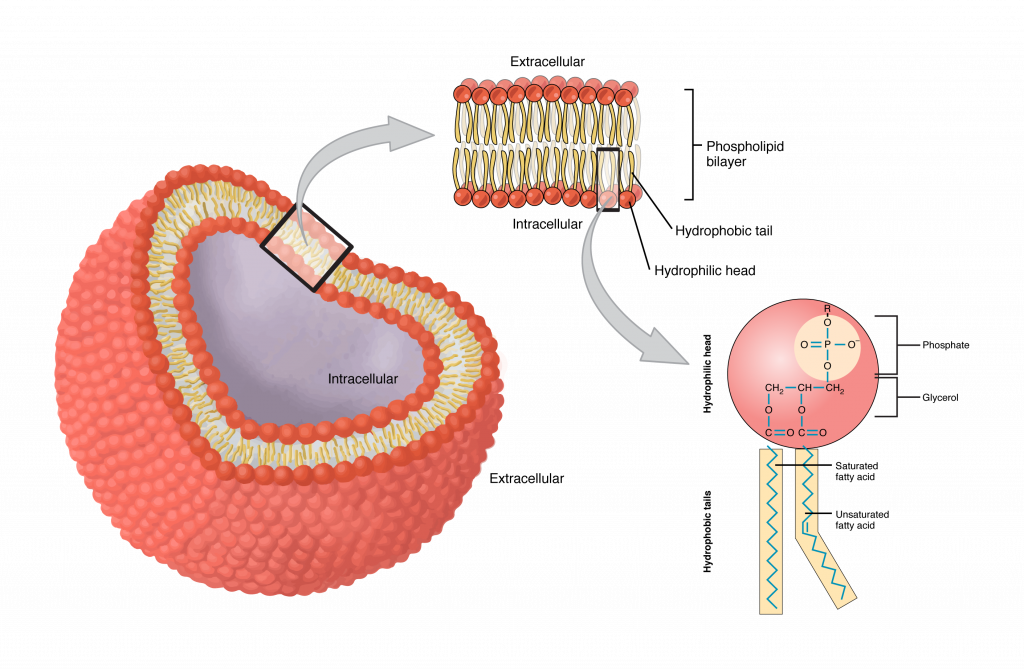
\includegraphics[width=.8\textwidth]{fig/phospholipid1.png}
\caption{\label{fig:LipidSphere}
\href{https://open.oregonstate.education/aandp/chapter/3-1-the-cell-membrane}{A simulated picture of the neuron membrane}.
We can consider the membrane as a closed surface (in our idealist view, a sphere), being slightly opened at an attached tube, the axon. For certain processes, we can also consider just a tiny section as a planar piece, see also Figure~\ref{fig:MembraneSurface}
}	
\end{figure}


\begin{figure}
\centering
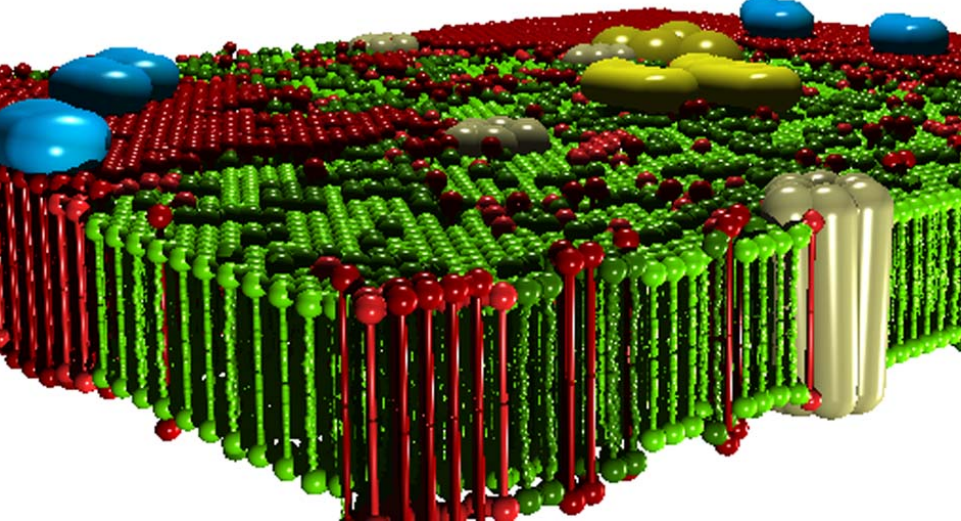
\includegraphics[width=.65\textwidth]{fig/HeimburgMembrane.png}
\caption{\label{fig:MembraneSurface}
A closer look at the simulated picture of the neuron membrane
shown in Fig.~\ref{fig:LipidSphere}.
Even the abstract model cannot stick to the flat surface
and the uniform membrane thickness. In addition, lipids spontaneously form double layers; moreover, smaller biological objects can build up on the membrane.
Lipids are amphiphilic molecules that like water on one side and repel water
on the other side due to the hydrocarbon chains. In contact to
water lipids spontaneously form double layers  that are the basic building blocks of biomembranes.
}	
\end{figure}


\else


\begin{figure}
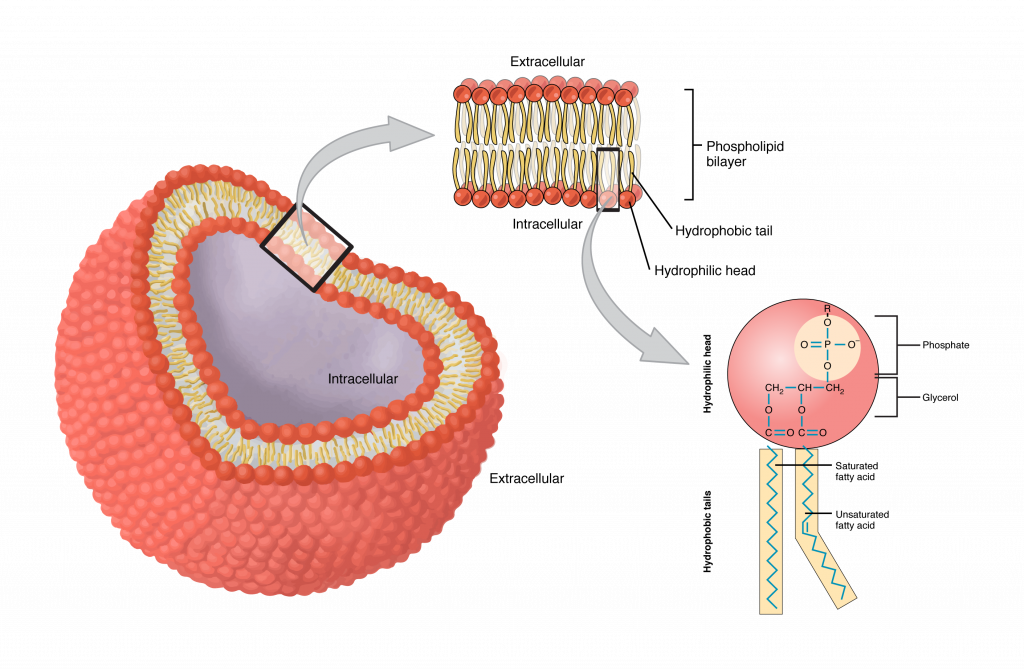
\includegraphics[width=.7\textwidth]{fig/phospholipid1.png}
\caption{\label{fig:LipidSphere}
\href{https://open.oregonstate.education/aandp/chapter/3-1-the-cell-membrane}{A neuron membrán egy idealizált képe}.
A membránt egy zárt felületnek (ideális esetben gömbnek) tekintjük,
amelyet egy hozzá csatlakozó cső (az axon) tesz nyitottá. 
Bizonyos folyamatok esetén a membrán egy kis darabját síknak tekintjük, lásd a~\ref{fig:MembraneSurface} ábrát.
}	
\end{figure}
 
Leírásunkban a neuront szigetelőből (lipid kettősrétegből) készült zárt felületnek (ideális esetben: gömbnek) tekintjük (a membrán), lásd \ref{fig:LipidSphere}~ábra, amelyhez egy ugyanolyan kivezető cső (az axon) csatlakozik, lásd \ref{fig:MembraneSurface}~ábra.
Mindkettő sóoldattal van töltve, és egy másfajta összetételű
sóoldat veszi körbe. A működéséhez kapcsolódó folyamatokban 
pedig kis darabkáját sík felületnek tekintjük (lásd ~\ref{fig:MembraneSurface} ábra), amely sajátos struktúrával 
rendelkezik ugyan, de számunkra csak a két sóoldatot
összekötő protein betét nyílások (az ioncsatornák)
és a más neuronok axonjainak az adott neuronhoz vezető
végződései (a szinapsisok) fontosak.
A neuront tehát olyan önálló biológiai objektumnak tekintjük,
amelyik állapotát saját szabályzó rendszerrel állítja be
és tartja meg, állapotára közvetlen külső környezete az ioncsatornákon keresztül hat. Más neuronokkal az axonokon
keresztül tart kapcsolatot: neurális impulzusokat küld és fogad.



\begin{figure}
\centering
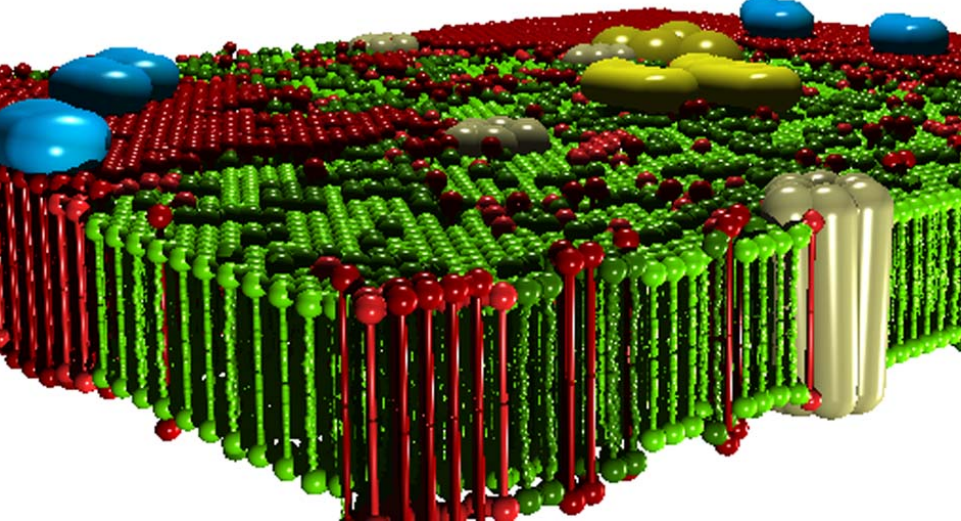
\includegraphics[width=.65\textwidth]{fig/HeimburgMembrane.png}
\caption{\label{fig:MembraneSurface}
A neuron membrán közelebbről.
Még az absztakt modell sem ragaszkodhat ahhoz, hogy a membrán 
felülete sík és a vastagsága egyenletes.
A membránok spontán módon alkotnak kettős rétegeket; azonban kisebb
biológiai objektumok rakódhatnak le a felszínükön.
A lipidek szénhirogén láncai egyik oldalukon emkötik, másik oldalukon
taszítják a vízmolekulákat.
Az ilyen rétegek a biomembránok alapvető építőkövei.
}	
\end{figure}
\fi



\ifx\magyar\undefined

In the case of mathematical modeling, we describe the measured data recorded about the phenomena on a "looks like" basis with a mathematical function (HH published \textit{quantified measurement results} in their own opinion), and possibly some ad-hoc assumed physical mechanism is put behind it.
In the case of physical modeling, we reduce the unknown operation in question to something that we already know, whose behavior we see as similar to that of the object under investigation in some respect, and whose mathematical description we can handle. Of course, similarity has limits, especially if we try to model a living object with an inanimate object described by the disciplinary methods of science. Based on the model, we can not only find limitations, but also how we can make our model more accurate; even if this requires combining the disciplines of inanimate natural science.

In the case of a living neuron, we can find many similarities with the functioning of an inanimate object: "whose thoughts come to mind" obviously means that the previous or even the most recent knowledge and available tools of the investigating scientist can decisively determine the scope of the modeling phenomenon. HH's work is hardly independent of the radar development work they carried out during the war years.
Similarly, when developing the model they proposed,
they took into account that the computational capacity at their disposal was a mechanical ("winding") computer. Unfortunately, their descriptions, which contained strongly simplifying assumptions, were encoded in the form of coefficients; thus, our modern calculations on advanced computers are based on them.

\else
Matematikai modellezés esetén a jelenségekről rögzített mérési adatokat "looks like" alapon leírjuk matematikai függvénnyel (HH saját véleménye szerint kvantitatizált mérési eredményeket tett közzé), és esetlegesen valami ad-hoc feltételezett fizikai mechanizmust állítunk mögé.
Fizikai modellezés esetén a tekintett ismeretlen működést olyanra vezetjük vissza, amit már ismerünk, viselkedését valamilyen szempontból a vizsgált objektuméhoz hasonlónak látjuk, és aminek matematikai leírását kezelni tudjuk. Természetesen a hasonlóságnak korlátai vannak, különösen ha élő objektumot próbálunk a tudomány diszciplináris módszereivel leírt élettelen objektummal modellezni. A modell alapján nem csak korlátokra jöhetünk rá, hanem arra is, hogy modellünket hogyan tudjuk pontosabbá tenni; még akkor is, ha ezzel az élettelen természettudomány diszciplináit kombinálni kell.

Az élő neuron esetén számos hasonlóságot találhatunk egy-egy élettelen objektum működésével: a "kinek mi jut róla eszébe" nyilván azzal jár, hogy a vizsgálódó tudós korábbi vagy éppen legfissebb  ismeretei, rendelkezésre álló eszközei akár döntően meghatározzák a modellezés jelenségkörét. \gls{HH} munkája aligha független a háborús években végzett radar fejlesztési munkáiktól.
Hasonlóképpen, az általuk javasolt modell kidolgozásakor
figyelembe vették, hogy a rendelkezésükre álló számítási kapacitás egy mechanikus ("tekerős") számítógép volt. Sajnos, erőteljesen egyszerűsítő feltevéseiket tartalmazó leírásaikat együtthatók formájában kódolták; így a fejlett számítógépeken futó mai számításaink is ezeken alapulnak. 

\fi

\ifx\magyar\undefined
The theory describing its operation must answer questions such as
\begin{itemize} 
\setlength\itemsep{0em}

\item why a resting potential exists
\item why the experienced ionic currents exist even in the so-called stable resting state
\item why this state changes to an unstable transient state
\item why the neuron can return to the same stable resting state
\item why it can turn to a transient state again before reaching the resting state
\item why there is a dead time before it can return to a transient state
\item why the parameters of the transient state are constant
\item why exactly such parameters describe the wave emitted in the transient state
\item how the emitted wave can propagate practically without attenuation
\end{itemize}

\else

A működést leíró elméletnek választ kell adni olyan kérdésekre, hogy
\begin{itemize}
\item miért létezik nyugalmi potenciál
\item miért léteznek a tapasztalt
ionáramok még a stabilnak mondott nyugalmi helyzetben is
\item miért változik meg ez az állapot egy instabil tranziens
állapotra
\item miért tud a neuron visszatalálni ugyanabba a
stabil nyugalmi állapotba
\item miért tud még a nyugalmi állapot elérése előtt
újból tranziens állapotba kerülni
\item miért van egy holtidő, amíg nem képes újból   tranziens állapotba kerülni
\item miért állandóak a tranziens állapot paraméterei
\item miért pont olyan paraméterek írják le a tranziens állapotban kibocsátott hullámot
\item hogyan tud a kibocsátott hullám gyakorlatilag gyengítés nélkül terjedni
\end{itemize}
\fi

%The membrane functions as a \hyperlink{ControlTheory}{\gls{PID} control circuit}.
\ifx\magyar\undefined
\subsection[Neuron's states]{Neuron's states \label{sec:Model-NeuronStates}}
\else
\subsection[A neuron állapotai]{A neuron állapotai\label{sec:Model-NeuronStates}}
\fi

\ifx\magyar\undefined
Under a small external influence, a neuron remains in its resting state and regulates itself through non-controlled ion channels in its membrane.
If the external influence exceeds a threshold, the controlled channels in the wall suddenly release a large amount of ions into the internal space, putting the neuron into a transient state.
The membrane potential changes suddenly (within a few dozen nanoseconds), and, due to the mutual repulsion of ions, the pressure acting on the membrane wall and the ion concentration in the layer near the membrane also increase significantly and suddenly. At this point, the disciplines of electricity and thermodynamics can be combined: the pressure and the electric field are proportional to the number of ions in the volume.
The forces exerted on ions, calculated in a disciplinary way, are falsified 
in the sense that the other discipline also contributes inseparably; in a strict sense, neither of the two disciplines alone can describe ions' motion.
The detailed analysis shows that the elastic energy during the action potential
is about two orders of magnitude higher than the electrical energy, but the 
amount of ions is about three oders of magnitude lower than that of the non-dissociated molecules.
It that situation, the two effects are of the same order of magnitude,
so that they can modulate each other. The electric charge on the membrane's wall 
would produce a simple discharge current. However, its charge carriers are
delivered by the damped oscillation of the electrolyte (a soliton) generated by the membrane.
The amplitude of the soliton changes the number of the charge carriers delivered,
so physiology measures an oscillating discharge current (that generates
a potential wave known as \gls{AP}). No significant mass transfer
takes place.

\else

Kis külső behatás esetén, a neuron nyugalmi állapotában marad és szabályozza állapotát a falban levő vezérletlen ioncsatornákon át.
Ha a külső behatás túllép egy küszöbértéket, a falban levő vezérelt 
ioncsatornákon át nagy mennyiségű ion kerül a belső térbe,
és a neuron tranziens állapotba kerül.
A membrán potenciál értéke hirtelen (néhány tucat nanosecundum alatt)
megváltozik, és, az ionok kölcsönön taszítása miatt, megnő a
membrán falra ható nyomás; továbbá, az ionok egyidejűleg megnövelik 
a membrán-közeli rétegekben a koncentrációt.
Ezen a ponton lehet kombinálni az elektromosságtan és a termodinamika
diszciplináit: a nyomás és az elektromos tér egyránt a térfogatrészben
található ionok számával arányos.
Az ionokra ható, diszciplináris módon számított erők olyan értelemben
nem valódiak, hogy a másik diszciplina következtében elválaszthatatlanul fellépő erők összeadódnak; szigorúan véve, egyik diszciplina sem tudja
leírni az ion mozgását: az általa ismert erő alapján az ion mozgásának nem olyannak kell lenni. 
A részletes analízis azt mutatja, hogy az \gls{AP} során a
rugalmas energia körülbelül két nagyságrenddel nagyobb,
mint az elektromos energia; viszont az ionok száma kb. három nagyságrenddel kisebb, mint a nem disszociált molekuláké.
%The detailed analysis shows that the elastic energy during the action potential
%is about two orders of magnitude higher than the electrical energy, but the 
%amount of ions is about three oders of magnitude lower than that of the non-dissociated molecules.
Ebben a helyzetben a két hatás ugyanabba a nagyságrendbe esik,
így modulálni tudják egymást.
Az elektromos kisülés egy egyszerű kisülési áramot jelentene.
Azonban, az elektrolitnak a membrán által generált rezgőmozgása (a soliton) szállítja a töltéshordozókat.
A soliton amplitúdója változtatja a szállított töltéshordozók számát,
így a fiziológiai elektromos mérés egy oszcilláló kisülési áramot
érzékel (ami az \gls{AP} néven ismert potenciálhullámot generálja).
A jelenség során nincs jelentős tömeg átvitel.
\fi

\ifx\magyar\undefined


Fig.~\ref{fig:NeuronStateMachine} illustrates our abstract view of a neuron,
in this case as a "stage machine".
Notice that the double circles are \textit{stages} (\textit{states} with event-defined periods) connected 
by bent arrows representing \textit{instant stage transitions}, while at some other abstraction level we consider them as \textit{processes} having a temporal course
with their own \textit{event} handling. Fundamentally, the system is circulating along the blue pathway, and maintains its state by using 
the black loops, but sometimes it takes the less common red pathways.
It reveives its inputs cooperatively
(controls the accepted amount of its external inputs from the upstream neurons by gating them by regulating a stage variable), furthermore
it actively communicates \textit{the time of its state change} (that is: \textit{not its state} as assumed in the so called neural information theory) toward the downstream neurons in a process
parallel with its mentioned activity.
\else
\fi

\ifx\magyar\undefined

\subsection[Stages]{Stages of operation\label{sec:Single-OperationStages}}
\else

\subsection[Fázisok]{A működés fázisai\label{sec:Single-OperationStages}}
\fi

\ifx\magyar\undefined


Initially, a neuron is in stage "Relaxing" which is the ground state of its operation.
(We also introduce a "Sleeping" or "Standby" helper stage, which can be imagined 
as a low-power mode in electronical or state maintenance mode of biological  computing; or "creating the neuron" in biology; a "no payload activity" stage.) The stage transition from "Sleeping" also \textit{resets the internal stage variable} membrane potential (to the value of the resting potential).
In biology, a "leakage" background activity takes place: it changes (among others) the stage variable towards the system's "no activity" value.

\begin{figure*}
\centering
\iflatexml
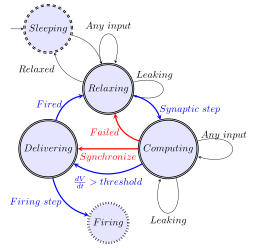
\includegraphics[width=.75\textwidth]{fig/NeuronStateMachineSimple.svg}
\else
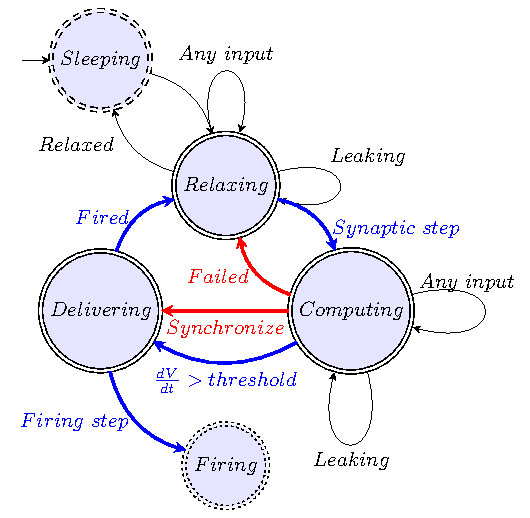
\includegraphics[width=0.65\textwidth]{fig/NeuronStateMachineSimple.pdf}
\fi
		\caption{The model of neuron as an abstract state machine\label{fig:NeuronStateMachine}}
\end{figure*} 

\else


Initially, a neuron is in stage "Relaxing" which is the ground state of its operation.
(We also introduce a "Sleeping" or "Standby" helper stage, which can be imagined 
as a low-power mode in electronical or state maintenance mode of biological  computing; or "creating the neuron" in biology; a "no payload activity" stage.) The stage transition from "Sleeping" also \textit{resets the internal stage variable} membrane potential (to the value of the resting potential).
In biology, a "leakage" background activity takes place: it changes (among others) the stage variable towards the system's "no activity" value.

\begin{figure*}
\iflatexml
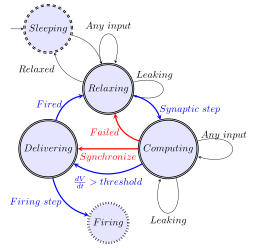
\includegraphics[width=.75\textwidth]{fig/NeuronStateMachineSimple.svg}
\else
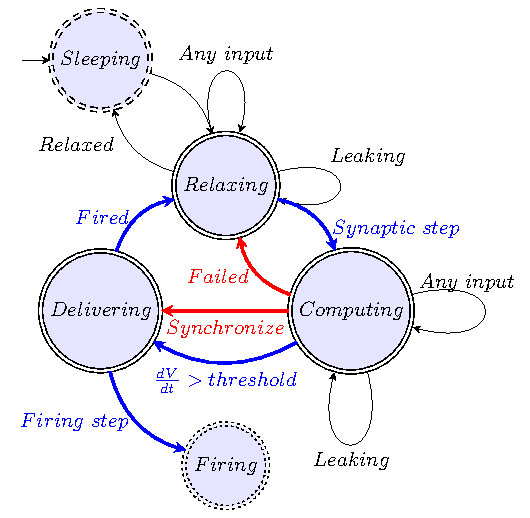
\includegraphics[width=0.65\textwidth]{fig/NeuronStateMachineSimple.pdf}
\fi
		\caption{The model of neuron as an abstract state machine\label{fig:NeuronStateMachine}}
\end{figure*} 


\fi


\ifx\magyar\undefined

An event (in form of a pulse of slow ions) arriving from the environment acts as a "look at me" signal
\index{slow current}
and the system passes to "Computing" stage: an excitation begins.
The external signal
acts as triggering a stage change and, simultaneously, contributes to the value of the internal stage variable (membrane voltage).
During normal operation, when the stage variable reaches the critial value (the threshold potential),
the system generates an event: passes to stage "Delivering" and "flushes" the collected charge.
In that stage, it starts to deliver a signal toward the environment
(to  the other neurons connected to its axon) and after a fixed period, passes to stage "Relaxing",
without resetting the stage variable. From this event on, it is again in stage
"Relaxing", where the "leakage" and the input pulses from the upstream neurons contribute to its
stage variable. Process "Delivering" operates an independent subsystem ("Firing"): happens simultaneously with 
process of "Relaxing" which, after some time, usually passes to the next "Computing".

\textit{The stages "Computing" and "Delivering" mutually block 
each other and the I/O operations happen in parallel with them}. They have temporal lengths, and they must follow in the well-defined order (a "proper sequencing"~\cite{EDVACreport1945,VeghRevisingClassicComputing:2021}) "Computing"$\Rightarrow$ "Delivering"$\Rightarrow$"Relaxing". Theoretically, \textit{a three-state system is needed to define the direction of time}~\cite{ThreeStateUnidirectional:2004}; a fundamental issue for quantum-based computing is the lack of a third state. In electronical computing we can introduce this as "up" edge and "down" edge, with a "hold" stage between.  A charge-up process must always happen before discharging. Stage "Delivering" has a fixed period, stage "Computing" has a variable period (depends mainly on the upstream neurons), and the total length of the computing period equals their sum. The (physiologically defined) length of the "Delivering" period limits neuron's firing rate; the length of "Computing" is usually much shorter.

\else

An event (in form of a pulse of slow ions) arriving from the environment acts as a "look at me" signal
\index{slow current}
and the system passes to "Computing" stage: an excitation begins.
The external signal
acts as triggering a stage change and, simultaneously, contributes to the value of the internal stage variable (membrane voltage).
During normal operation, when the stage variable reaches the critial value (the threshold potential),
the system generates an event: passes to stage "Delivering" and "flushes" the collected charge.
In that stage, it starts to deliver a signal toward the environment
(to  the other neurons connected to its axon) and after a fixed period, passes to stage "Relaxing",
without resetting the stage variable. From this event on, it is again in stage
"Relaxing", where the "leakage" and the input pulses from the upstream neurons contribute to its
stage variable. Process "Delivering" operates an independent subsystem ("Firing"): happens simultaneously with 
process of "Relaxing" which, after some time, usually passes to the next "Computing".

\textit{The stages "Computing" and "Delivering" mutually block 
each other and the I/O operations happen in parallel with them}. They have temporal lengths, and they must follow in the well-defined order (a "proper sequencing"~\cite{EDVACreport1945,VeghRevisingClassicComputing:2021}) "Computing"$\Rightarrow$ "Delivering"$\Rightarrow$"Relaxing". Theoretically, \textit{a three-state system is needed to define the direction of time}~\cite{ThreeStateUnidirectional:2004}; a fundamental issue for quantum-based computing is the lack of a third state. In electronical computing we can introduce this as "up" edge and "down" edge, with a "hold" stage between.  A charge-up process must always happen before discharging. Stage "Delivering" has a fixed period, stage "Computing" has a variable period (depends mainly on the upstream neurons), and the total length of the computing period equals their sum. The (physiologically defined) length of the "Delivering" period limits neuron's firing rate; the length of "Computing" is usually much shorter.

\fi

\ifx\magyar\undefined


In any stage, a "leak current" (through ion channels, but mainly the \gls{AIS}
instead of the membrane)
changing the stage variable is present; \textbf{\textit{the continuous change (the presence of a voltage gradient) has a fundamental importance for a biological computing system}}
 \index{voltage gradient}
This current is proportional to the stage variable (membrane current); it is \textbf{\textit{not}} identical with the fixed-size "leak current" assumed in the Hodgkin-Huxley model~\cite{HodgkinHuxley:1952}.
The event which is issued when stage "Computing" ends and "Delivering" begins, separates two physically different operating modes: inputting payload signals for computing
and inputting "servo" ions for transmitting
(signal transmission to fellow neurons begins and happens in parallel
with further computation(s)).
Given that stages "Computing" and "Delivering" take time,
and the next "Computing" can only start through the stage "Relaxing",   
furthermore "Delivering" can only begin after "Computing" finished,
\textit{these stages mutually block each other} (and the length of the "Delivering" period limits neuron's firing rate). 

There are two more possible stage transitions from the stage "Computing".
First, the stage variable (due to "leaking") may approach its initial value (the resting potential) without firing and the system passes to stage "Relaxing"; in this case we consider that the excitation "Failed".
This happens when leaking is more intense than the input current pulses (the input firing rate is too low or a random firing event started the computing).
Second, an external pulse may have the effect to force the system (independently from the value of the stage variable) to pass instantly to stage "Delivering", and after that, to "Relaxing". (When several neurons share that input signal,
they will go to "Relaxing" at the same time: they get synchronized; a simple way of synchronizing low-precision asynchronous oscillators.)


\else

In any stage, a "leak current" (through ion channels, but mainly the \gls{AIS}
instead of the membrane)
changing the stage variable is present; \textbf{\textit{the continuous change (the presence of a voltage gradient) has a fundamental importance for a biological computing system}}
 \index{voltage gradient}
This current is proportional to the stage variable (membrane current); it is \textbf{\textit{not}} identical with the fixed-size "leak current" assumed in the Hodgkin-Huxley model~\cite{HodgkinHuxley:1952}.
The event which is issued when stage "Computing" ends and "Delivering" begins, separates two physically different operating modes: inputting payload signals for computing
and inputting "servo" ions for transmitting
(signal transmission to fellow neurons begins and happens in parallel
with further computation(s)).
Given that stages "Computing" and "Delivering" take time,
and the next "Computing" can only start through the stage "Relaxing",   
furthermore "Delivering" can only begin after "Computing" finished,
\textit{these stages mutually block each other} (and the length of the "Delivering" period limits neuron's firing rate). 

There are two more possible stage transitions from the stage "Computing".
First, the stage variable (due to "leaking") may approach its initial value (the resting potential) without firing and the system passes to stage "Relaxing"; in this case we consider that the excitation "Failed".
This happens when leaking is more intense than the input current pulses (the input firing rate is too low or a random firing event started the computing).
Second, an external pulse may have the effect to force the system (independently from the value of the stage variable) to pass instantly to stage "Delivering", and after that, to "Relaxing". (When several neurons share that input signal,
they will go to "Relaxing" at the same time: they get synchronized; a simple way of synchronizing low-precision asynchronous oscillators.)


\fi

\ifx\magyar\undefined

Anyhow: a neuron operates in cooperation with in its environment (the fellow neurons, with outputs distributed in space and time).
It receives multiple inputs at different times (at different offset times from the different upstream neurons) and in different stages. 
In stage "Computing", the synaptic inputs are open, while
in stage "Delivering", the synaptic inputs are closed (the input is ineffective).
It produces multiple outputs (in the sense that the signal may branch along its path), in form of a signal with temporal course.
\else

Anyhow: a neuron operates in cooperation with in its environment (the fellow neurons, with outputs distributed in space and time).
It receives multiple inputs at different times (at different offset times from the different upstream neurons) and in different stages. 
In stage "Computing", the synaptic inputs are open, while
in stage "Delivering", the synaptic inputs are closed (the input is ineffective).
It produces multiple outputs (in the sense that the signal may branch along its path), in form of a signal with temporal course.
\fi


\ifx\magyar\undefined
 

%\subsection[Overview]{Overview of stages\label{sec:Single-StagesOverview}}


\subsubsection[Computing]{Stage 'Computing'\label{sec:Single-OperationComputing}}
%\subsubsection{Stage 'Computing'\label{sec:Single-OperationComputing}}

\else
 

%\subsection[Overview]{Overview of stages\label{sec:Single-StagesOverview}}


\subsubsection[Computing]{Stage 'Computing'\label{sec:Single-OperationComputing}}
%\subsubsection{Stage 'Computing'\label{sec:Single-
\fi

\ifx\magyar\undefined


The neuron receives its inputs as 'Axonal inputs'. For the first input in stage 'Relaxing',
the neuron enters stage 'Computing'. 
The  time of this event is the base time used for calculating the neuron's "local time" (in describing the operation and in the simulator). 
\index{local time}
Notice that producing the result is a cooperation 
between the neuron and its upstream neurons (the neuron gates its input currents). One of the upstream neurons
opens computing, and the receiving neuron terminates it.


The physical implementation is
a steep current gradient which evokes a steep \hyperlink{voltage_gradient}{voltage gradient} $dV/dt$
on the condenser 'membrane' in its intracellular segment, see section~\ref{subsec:Single-PSP}. 
\index{voltage gradient}
The membrane is connected to the axon through a resistor 
%\gls{AIS}
'AIS'
(these components, switched in serial, constitute the \hyperlink{PhysicsOscillator}{neuronal oscillator}).
Given that the current creates a potential gradient on the membrane, the 
increased potential starts a current ("Leaking") proportional to the voltage difference
between the membrane and the axon (across the AIS). This current decreases
the membrane's potential (discharges the condenser). In lack of further 
excitation, the membrane's potential decreases back to its resting value
and the neuron returns to stage 'Relaxing'.

\else


The neuron receives its inputs as 'Axonal inputs'. For the first input in stage 'Relaxing',
the neuron enters stage 'Computing'. 
The  time of this event is the base time used for calculating the neuron's "local time" (in describing the operation and in the simulator). 
\index{local time}
Notice that producing the result is a cooperation 
between the neuron and its upstream neurons (the neuron gates its input currents). One of the upstream neurons
opens computing, and the receiving neuron terminates it.


The physical implementation is
a steep current gradient which evokes a steep \hyperlink{voltage_gradient}{voltage gradient} $dV/dt$
on the condenser 'membrane' in its intracellular segment, see section~\ref{subsec:Single-PSP}. 
\index{voltage gradient}
The membrane is connected to the axon through a resistor 
%\gls{AIS}
'AIS'
(these components, switched in serial, constitute the \hyperlink{PhysicsOscillator}{neuronal oscillator}).
Given that the current creates a potential gradient on the membrane, the 
increased potential starts a current ("Leaking") proportional to the voltage difference
between the membrane and the axon (across the AIS). This current decreases
the membrane's potential (discharges the condenser). In lack of further 
excitation, the membrane's potential decreases back to its resting value
and the neuron returns to stage 'Relaxing'.

\fi

\ifx\magyar\undefined

%
However, for repeated excitation, when the next 'Axonal input' arrive(s) before
the neuron returns to stage 'Relaxing', the voltage increases further, and it might reach
a threshold voltage. In such a case, the neuron enters stage 'Delivering'
(the red section of the broken diagram line). The time at which point this happens
depends on the arrival of spikes and the discharge of the membrane (when the
difference of the received charge and the loss due to discharge evokes
a sufficiently large voltage on the condenser's capacity). At that point,
the computation is finished. \textit{The result of the computation is
the time} passed between receiving the first 'Axonal input' and the time when
the neuron closes its input sources (and simultaneously, opens the ion channels
in its wall, see below, to enter stage "Delivering").  No more input shall be received, so
the neuron disables its synaptic inputs, and prepares for delivering 
the result of its 'computation' (nothing shall be stored: the result is the time of sending the message, but the delivery period takes time; is a fixed-length
process, will follow immediately). 
In this stage, the role of the slow speed is not evident. The current 
arrives through an axon, passes the terminal and arrives at the AIS;
the time components cannot be separated. 

\else

However, for repeated excitation, when the next 'Axonal input' arrive(s) before
the neuron returns to stage 'Relaxing', the voltage increases further, and it might reach
a threshold voltage. In such a case, the neuron enters stage 'Delivering'
(the red section of the broken diagram line). The time at which point this happens
depends on the arrival of spikes and the discharge of the membrane (when the
difference of the received charge and the loss due to discharge evokes
a sufficiently large voltage on the condenser's capacity). At that point,
the computation is finished. \textit{The result of the computation is
the time} passed between receiving the first 'Axonal input' and the time when
the neuron closes its input sources (and simultaneously, opens the ion channels
in its wall, see below, to enter stage "Delivering").  No more input shall be received, so
the neuron disables its synaptic inputs, and prepares for delivering 
the result of its 'computation' (nothing shall be stored: the result is the time of sending the message, but the delivery period takes time; is a fixed-length
process, will follow immediately). 
In this stage, the role of the slow speed is not evident. The current 
arrives through an axon, passes the terminal and arrives at the AIS;
the time components cannot be separated. 

\fi

\ifx\magyar\undefined


\subsubsection[Delivering]{Stage 'Delivering'\label{sec:Single-OperationDelivering}}

\else


\subsubsection[Delivering]{Stage 'Delivering'\label{sec:Single-OperationDelivering}}

\fi

\ifx\magyar\undefined

In this stage,
the result is ready: the time between the arrival of the first
synaptic input and reaching the membrane's threshold voltage is measured.
No more input is desirable, so the neuron's input synapses remain closed.
Simultanously, the neuron starts it "servo" mechanism: it opens its ion channels
and an intense ion current starts to charge the membrane. 
It is an 'instant' current.
The voltage on the membrane quickly rises, but it takes a short time
until its peak voltage reached.
Given that the charge-up current is instant and the increased
membrane voltage drives an outward current, the membrane voltage
gradually decays.
When the voltage drops below the threshold voltage, the neuron re-opens its synaptic inputs and passes to stage "Relaxing": it is ready for the next operation. The signal transmission to downstream neurons
happens in parallel with the recent "Delivering" stage and
the next "Relaxing" and maybe "Computing" stages. 
%The actual electric operation is discussed in section~\ref{sec:Physics-OperationDelivering}.

Delivering the result needs huge power because of the noisy environment and 
the huge distances, so at the beginning of the 'Delivery' phase,
the neuron switches in a 'servo' mechanism. Exceeding the threshold voltage
(either as a consequence of the 'spatiotemporal' summing several spikes or a single spike with sufficiently large voltage gradient~\cite{LosonczyIntegrative:2006}) opens the voltage-gated ion channels in the membrane's wall. 
Due to the
vast voltage gradient across the two segments of the membrane, an enormous 
amount of ions rush-in into the intracellular space and the intense current
increases the membrane's potential; for the details see section~\ref{sec:Physics-Electricity}. The amount of the rushed-in ions
is several times more than those received during the stage 'Computing'.

\else

In this stage,
the result is ready: the time between the arrival of the first
synaptic input and reaching the membrane's threshold voltage is measured.
No more input is desirable, so the neuron's input synapses remain closed.
Simultanously, the neuron starts it "servo" mechanism: it opens its ion channels
and an intense ion current starts to charge the membrane. 
It is an 'instant' current.
The voltage on the membrane quickly rises, but it takes a short time
until its peak voltage reached.
Given that the charge-up current is instant and the increased
membrane voltage drives an outward current, the membrane voltage
gradually decays.
When the voltage drops below the threshold voltage, the neuron re-opens its synaptic inputs and passes to stage "Relaxing": it is ready for the next operation. The signal transmission to downstream neurons
happens in parallel with the recent "Delivering" stage and
the next "Relaxing" and maybe "Computing" stages. 
%The actual electric operation is discussed in section~\ref{sec:Physics-OperationDelivering}.

Delivering the result needs huge power because of the noisy environment and 
the huge distances, so at the beginning of the 'Delivery' phase,
the neuron switches in a 'servo' mechanism. Exceeding the threshold voltage
(either as a consequence of the 'spatiotemporal' summing several spikes or a single spike with sufficiently large voltage gradient~\cite{LosonczyIntegrative:2006}) opens the voltage-gated ion channels in the membrane's wall. 
Due to the
vast voltage gradient across the two segments of the membrane, an enormous 
amount of ions rush-in into the intracellular space and the intense current
increases the membrane's potential; for the details see section~\ref{sec:Physics-Electricity}. The amount of the rushed-in ions
is several times more than those received during the stage 'Computing'.

\fi

\ifx\magyar\undefined


The ion channels over the surface of the neuron open
at the same time, and they are open only for a very short period
(actually, they implement a sudden "step current"). However, this 
current on the surface is created at different distances from the \gls{AIS}
and (due to the final speed of the ions) and the time until the ions 
arrive at the \gls{AIS} depends on the distance to \gls{AIS}.
Due to this effect, the current quickly increases;
until it reaches a maximum. 
The time when the \gls{AP} reaches maximum value (due to the event that
the current from the most distant places of the membrane could reach \gls{AIS}), 
and from this point it starts to decrease.
(there is no other special threshold voltage value:
the charge from the rush-in current distributes on the surface;
the current injection can charge the fixed capacity 
membrane to that voltage).
At this point the neuronal condenser is maximally depolarized.
\index{depolarization}

The neuronal condenser is loaded to its maximum, and the resistor (the \gls{AIS})
enables a current to flow out, so the condenser (the membrane) discharges (repolarizes).
Here enters into the picture that the neuron is resemblant to a serial oscillator.
The condenser stores the charge for some period, and releases it to the \gls{AIS}
at a later time. As a result, the direction of the current on the neuron's
membrane reverses, see the shape of the output voltage in table~\ref{tab:Electric_RCOscillator_Circuits}.
The essential difference between the serial and parallel $RC$ oscillators is
that the differentiator circuit can produce opposite voltage on its output
without assuming any additional mechanism, such as an outward current,
given that \textit{a current pulse has rising and falling edges which can natively produce 
positive and negative voltage derivatives}.
As the result of the process, the potential reaching the AIS goes to negative;
a phenomenon called hyperpolarization.
\index{hyperpolarization}

\else


The ion channels over the surface of the neuron open
at the same time, and they are open only for a very short period
(actually, they implement a sudden "step current"). However, this 
current on the surface is created at different distances from the \gls{AIS}
and (due to the final speed of the ions) and the time until the ions 
arrive at the \gls{AIS} depends on the distance to \gls{AIS}.
Due to this effect, the current quickly increases;
until it reaches a maximum. 
The time when the \gls{AP} reaches maximum value (due to the event that
the current from the most distant places of the membrane could reach \gls{AIS}), 
and from this point it starts to decrease.
(there is no other special threshold voltage value:
the charge from the rush-in current distributes on the surface;
the current injection can charge the fixed capacity 
membrane to that voltage).
At this point the neuronal condenser is maximally depolarized.
\index{depolarization}

The neuronal condenser is loaded to its maximum, and the resistor (the \gls{AIS})
enables a current to flow out, so the condenser (the membrane) discharges (repolarizes).
Here enters into the picture that the neuron is resemblant to a serial oscillator.
The condenser stores the charge for some period, and releases it to the \gls{AIS}
at a later time. As a result, the direction of the current on the neuron's
membrane reverses, see the shape of the output voltage in table~\ref{tab:Electric_RCOscillator_Circuits}.
The essential difference between the serial and parallel $RC$ oscillators is
that the differentiator circuit can produce opposite voltage on its output
without assuming any additional mechanism, such as an outward current,
given that \textit{a current pulse has rising and falling edges which can natively produce 
positive and negative voltage derivatives}.
As the result of the process, the potential reaching the AIS goes to negative;
a phenomenon called hyperpolarization.
\index{hyperpolarization}

\fi

\ifx\magyar\undefined

Notice that the current in the red section (plus also in the blue section) 
of the diagram line still originates from the rushed-in charge. The observer
sees the sum of the resistive and capacitive currents;
maybe new axonal inputs superimposed.
The ion current's finite speed plays again. When the axonal arbors re-open,
the ion flows into the membrane at some distant point, so its effect
will be observed some time later; apparently when the neuron membrane is
about its hyperpolarized state. 

\else

Notice that the current in the red section (plus also in the blue section) 
of the diagram line still originates from the rushed-in charge. The observer
sees the sum of the resistive and capacitive currents;
maybe new axonal inputs superimposed.
The ion current's finite speed plays again. When the axonal arbors re-open,
the ion flows into the membrane at some distant point, so its effect
will be observed some time later; apparently when the neuron membrane is
about its hyperpolarized state. 

\fi

\ifx\magyar\undefined


\subsubsection[Relaxing]{Stage 'Relaxing'\label{sec:Single-OperationRelaxing}}
\else

\subsubsection[Relaxing]{Stage 'Relaxing'\label{sec:Single-OperationRelaxing}}

\fi

\ifx\magyar\undefined


In this stage,
the neuron re-opens its synaptic gates. Recall that the ion channels
used for generating an intense membrane current
are already closed. The neuron passes to stage 'Relaxing' and is ready for a new computation:
the previous result is under delivering (parallelly, independently),
the axonal inputs are open again. 
However, the membrane's potential at this point may differ from the
resting potential.  A new computation begins
(the neuron passes to the stage "Computing")
when a new axonal input arrives.  Given that the computation is analog, a current flows through the AIS, and the result is the length of the period to reach
the threshold value, the 
membrane voltage plays the role of an accumulator (with a time-dependent content): a non-zero initial value acts as a short-time memory in the next computing cycle.
The local time is reset when a new computing cycle begins, but not when eventually the resting potential reached.
%The actual electric operation is discussed in section~\ref{sec:Physics-OperationRelaxing}.
\index{local time}

As the membrane's voltage drops below the threshold voltage,
the neuron re-opens its synaptic gates (the ion channels in the membrane's wall
are already closed). The neuron passes to stage 'Relaxing' and is ready for a new computation:
the previous result is under delivering (parallelly, independently),
the axonal inputs are open again. 
However, the membrane's potential at this point may differ from the
resting potential. Given that the computation is analog, the 
membrane voltage plays the role of an accumulator (with a time-dependent content,
given that the current flows though the AIS). A new computation begins
(the neuron passes to the stage "Computing")
when a new axonal input arrives. Given that the result is the time to reach
the threshold value, the non-zero initial value acts as a short-time memory.



The ion current's finite speed plays again. When the axonal arbors re-open,
the ion flows into the membrane at some distant point, so its effect
will be observed some time later; apparently when the neuron membrane is
about its hyperpolarized state. 
\else


In this stage,
the neuron re-opens its synaptic gates. Recall that the ion channels
used for generating an intense membrane current
are already closed. The neuron passes to stage 'Relaxing' and is ready for a new computation:
the previous result is under delivering (parallelly, independently),
the axonal inputs are open again. 
However, the membrane's potential at this point may differ from the
resting potential.  A new computation begins
(the neuron passes to the stage "Computing")
when a new axonal input arrives.  Given that the computation is analog, a current flows through the AIS, and the result is the length of the period to reach
the threshold value, the 
membrane voltage plays the role of an accumulator (with a time-dependent content): a non-zero initial value acts as a short-time memory in the next computing cycle.
The local time is reset when a new computing cycle begins, but not when eventually the resting potential reached.
%The actual electric operation is discussed in section~\ref{sec:Physics-OperationRelaxing}.
\index{local time}

As the membrane's voltage drops below the threshold voltage,
the neuron re-opens its synaptic gates (the ion channels in the membrane's wall
are already closed). The neuron passes to stage 'Relaxing' and is ready for a new computation:
the previous result is under delivering (parallelly, independently),
the axonal inputs are open again. 
However, the membrane's potential at this point may differ from the
resting potential. Given that the computation is analog, the 
membrane voltage plays the role of an accumulator (with a time-dependent content,
given that the current flows though the AIS). A new computation begins
(the neuron passes to the stage "Computing")
when a new axonal input arrives. Given that the result is the time to reach
the threshold value, the non-zero initial value acts as a short-time memory.



The ion current's finite speed plays again. When the axonal arbors re-open,
the ion flows into the membrane at some distant point, so its effect
will be observed some time later; apparently when the neuron membrane is
about its hyperpolarized state. 

\fi

\ifx\magyar\undefined

 
\subsubsection[Classic]{Classic stages\label{sec:Single-OperationClassicStages}}

\else

 
\subsubsection[Classic]{Classic stages\label{sec:Single-OperationClassicStages}}
\fi

\ifx\magyar\undefined


%We can map our 'modern' stages to those 'classic' stages and we can see
why defining the length of the Action Potential
%AP
is problematic.
The effect of slow current affects the apparent boundary between our
"Delivering" stage and "Relaxing" stages. 
Classical physiology sees the difference and distinguishes 'absolute' and 
'relative' refractory periods with a smeared boundary between. Furthermore,
it defines the length of the spike with some characteristic point,
such as reaching the resting value for the first or second time, or
reaching the maximum polarization/hyperpolarization.  Our derivation of the stages (see Fig.~\ref{fig:AP_Conceptual}) defines clear-cut breakpoints between them.

We can define the length of the spike as the sum of the variable-size length of period "Computing" and fixed-size period "Delivering". The "absolute refractory" 
period is defined as the period while the neuron membrane's voltage keeps
the gates of the synaptic inputs closed (the value of membrane voltage is above their threshold). That period is apparently extended 
(and interpreted as a "relative refractory" period, which sensitively depends
on the conduction velocity~\cite{APTemperatureDependenceRefractory:2001})
by the period when although the gating is re-enabled, but the slow current did not
yet arrive to the 
\gls{AIS}
where it contributes to the measured 
\gls{AP}, see Fig.~\ref{fig:AP_Conceptual}.  \textit{Only one refractory period exists,
plus the effect of the slow current.}
\index{refractory period}

\else


%We can map our 'modern' stages to those 'classic' stages and we can see
why defining the length of the Action Potential
%AP
is problematic.
The effect of slow current affects the apparent boundary between our
"Delivering" stage and "Relaxing" stages. 
Classical physiology sees the difference and distinguishes 'absolute' and 
'relative' refractory periods with a smeared boundary between. Furthermore,
it defines the length of the spike with some characteristic point,
such as reaching the resting value for the first or second time, or
reaching the maximum polarization/hyperpolarization.  Our derivation of the stages (see Fig.~\ref{fig:AP_Conceptual}) defines clear-cut breakpoints between them.

We can define the length of the spike as the sum of the variable-size length of period "Computing" and fixed-size period "Delivering". The "absolute refractory" 
period is defined as the period while the neuron membrane's voltage keeps
the gates of the synaptic inputs closed (the value of membrane voltage is above their threshold). That period is apparently extended 
(and interpreted as a "relative refractory" period, which sensitively depends
on the conduction velocity~\cite{APTemperatureDependenceRefractory:2001})
by the period when although the gating is re-enabled, but the slow current did not
yet arrive to the 
\gls{AIS}
where it contributes to the measured 
\gls{AP}, see Fig.~\ref{fig:AP_Conceptual}.  \textit{Only one refractory period exists,
plus the effect of the slow current.}
\index{refractory period}

\fi

\ifx\magyar\undefined
\subsection[Resting Potential]{Resting Potential\label{sec:Model-NeuronAbstractResting}}
\else
\subsection[Nyugalmi potenciál]{Nyugalmi potenciállabel{sec:Model-NeuronAbstractResting}}
\fi


                                                                           

\ifx\magyar\undefined
\subsection[Action Potential]{Action Potential\label{sec:Model-NeuronAbstractAction}}
\else
\subsection[Az akciós potenciál]{Az akciós potenciál\label{sec:Model-NeuronAbstractAction}}
\fi

\ifx\magyar\undefined

\begin{figure*}
\centering
\iflatexml
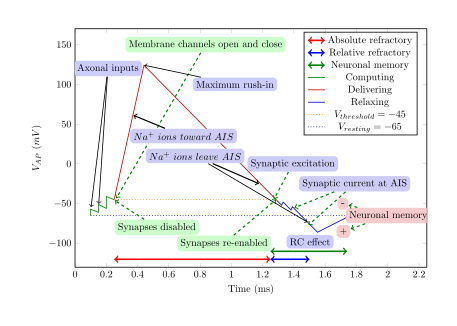
\includegraphics[width=\textwidth]{fig/AP_Schematic.svg}
\else
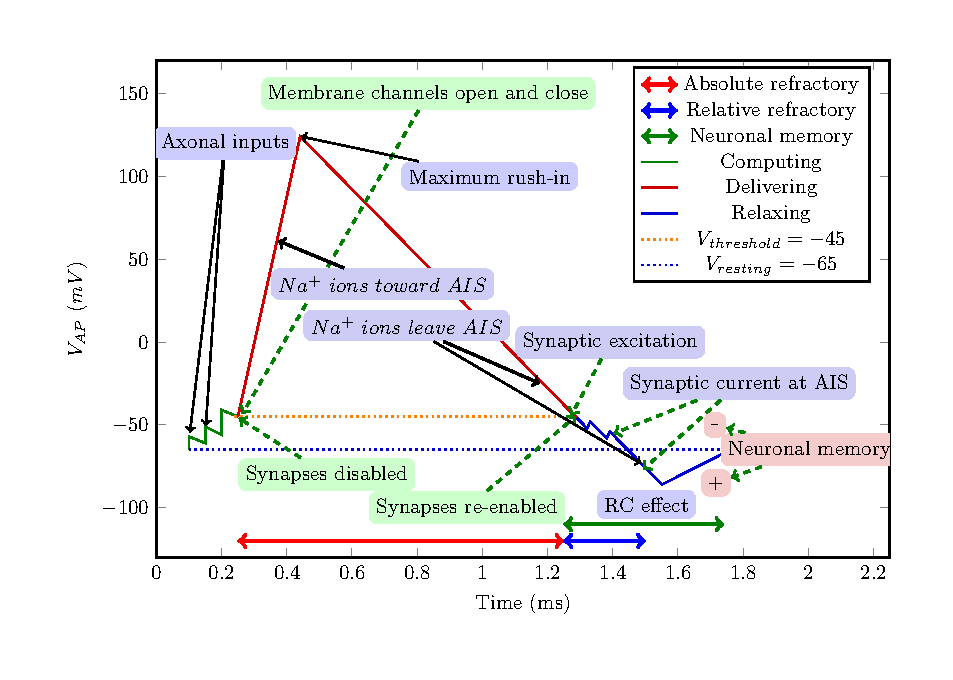
\includegraphics[width=.8\textwidth]{fig/AP_Schematic.pdf}
\fi
		\caption{The conceptual graph of the action potential \label{fig:AP_Conceptual}}
\end{figure*}   

\else
\begin{figure*}
\centering
\iflatexml
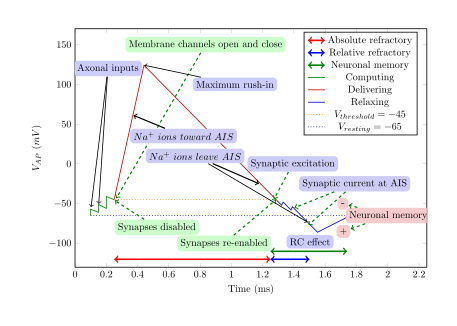
\includegraphics[width=\textwidth]{fig/AP_Schematic.svg}
\else
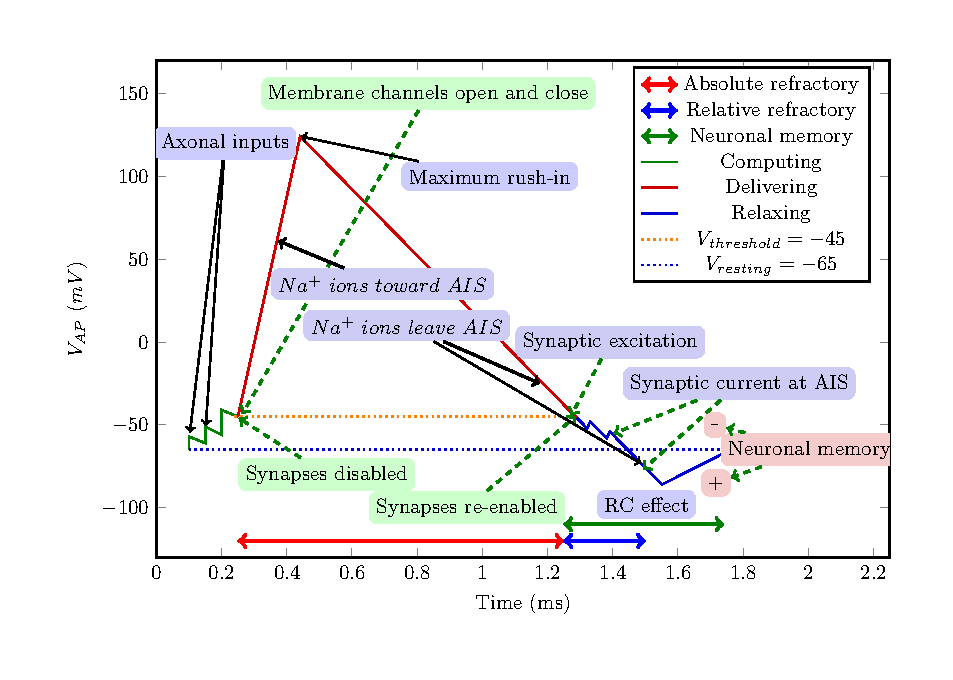
\includegraphics[width=.8\textwidth]{fig/AP_Schematic.pdf}
\fi
		\caption{Az akciós potenciál koncepciós diagramja \label{fig:AP_Conceptual}}

\fi


\ifx\magyar\undefined
\subsection[Neuron's control]{Neuron's control \label{sec:Model-NeuronControl}}

\else

\subsection[A neuron vezérlése]{A neuron vezérlése\label{sec:Model-NeuronControl}}
\fi

\ifx\magyar\undefined
Biology uses a simple \gls{PID} controller with proportional, integral, and derivative components. 
In simple words, it means that the output of the system (the output voltage measurable on the \gls{AIS}) depends on the input voltage (the present: input current if the resistance is constant),
the integrated input current(s) (the past), and their derivatives (the future). Notice that calculating the derivatives of the interdependent parameters needs care, as discussed in~\cite{MechanicalPropertiesNerves:2025}. The sum of those summands defines the resulting output voltage. 
The biological case is more complicated than the technical one because biology works with slow ions, and the components have
their temporal dependence (applying the laws created for fast currents requires emulation, as discussed in section~\ref{sec:Physics-FormingPotential}). Furthermore, the summands have several constituents, and the neurons handle those current-related constituents autonomously.
That is, unlike what is assumed in the classic physiology,
the output voltage is not necessarily a simple
function of the mentioned input variables.
Furthermore, it is not sufficient to consider the "present" of the system.
The classic models all omit the derivatives' contributions (a direct consequence of using 'clamping': in that "frozen" state, the "future" cannot be interpreted)
except that of the capacitive current, which is the passive consequence of the input currents.
Furthermore, the 'Integrate and Fire'-type models
consider the integrated currents only in the 'charge-up' ('Computing') period of operation, and they entirely omit that different physical processes are going on in different stages of operation.
That is, \textit{even the best classic models can not describe neuronal operation completely and correctly}.


The gradients are used to adjust the process variable through their positive and negative contributions (corresponding to rising and falling edges), and the different speeds of the thermodynamic and electrical interactions minimize the delay (i.e., provide the maximum operational speed, vital for survival).
The steady-state error is minimized by setting the process variable to the reference point using long-term stable parameters (geometry and overall concentration). The low-intensity current through the always-open resting ion channels provides dynamic stability in the steady state.%The permanently zero error signal indicates a lack of operations. 

\else

Biology uses a simple \gls{PID} controller with proportional, integral, and derivative components. 
In simple words, it means that the output of the system (the output voltage measurable on the \gls{AIS}) depends on the input voltage (the present: input current if the resistance is constant),
the integrated input current(s) (the past), and their derivatives (the future). Notice that calculating the derivatives of the interdependent parameters needs care, as discussed in~\cite{MechanicalPropertiesNerves:2025}. The sum of those summands defines the resulting output voltage. 
The biological case is more complicated than the technical one because biology works with slow ions, and the components have
their temporal dependence (applying the laws created for fast currents requires emulation, as discussed in section~\ref{sec:Physics-FormingPotential}). Furthermore, the summands have several constituents, and the neurons handle those current-related constituents autonomously.
That is, unlike what is assumed in the classic physiology,
the output voltage is not necessarily a simple
function of the mentioned input variables.
Furthermore, it is not sufficient to consider the "present" of the system.
The classic models all omit the derivatives' contributions (a direct consequence of using 'clamping': in that "frozen" state, the "future" cannot be interpreted)
except that of the capacitive current, which is the passive consequence of the input currents.
Furthermore, the 'Integrate and Fire'-type models
consider the integrated currents only in the 'charge-up' ('Computing') period of operation, and they entirely omit that different physical processes are going on in different stages of operation.
That is, \textit{even the best classic models can not describe neuronal operation completely and correctly}.


The gradients are used to adjust the process variable through their positive and negative contributions (corresponding to rising and falling edges), and the different speeds of the thermodynamic and electrical interactions minimize the delay (i.e., provide the maximum operational speed, vital for survival).
The steady-state error is minimized by setting the process variable to the reference point using long-term stable parameters (geometry and overall concentration). The low-intensity current through the always-open resting ion channels provides dynamic stability in the steady state.
\fi

\ifx\magyar\undefined
\begin{figure}
\centering
	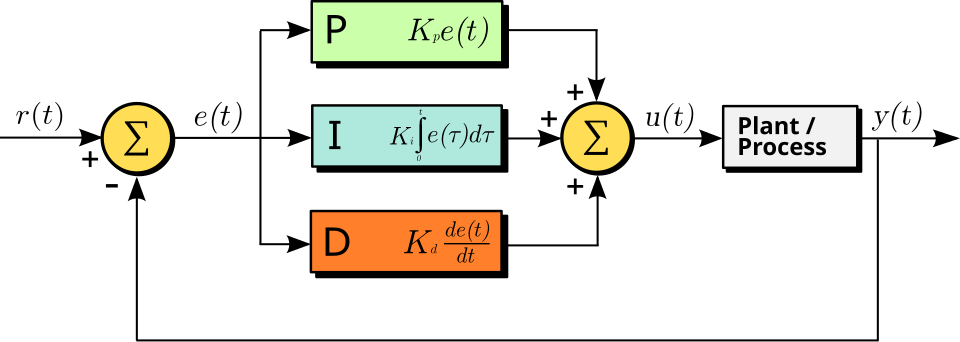
\includegraphics[width=0.8\columnwidth]{fig/PID_en.png}
	\caption{A block diagram of a PID controller in a feedback loop. r(t) is the desired process variable (PV) or setpoint (SP), and y(t) is the measured PV. (Wikipedia)\label{fig:PID_Controller}
	}
\end{figure}

\else

\begin{figure}
\centering
	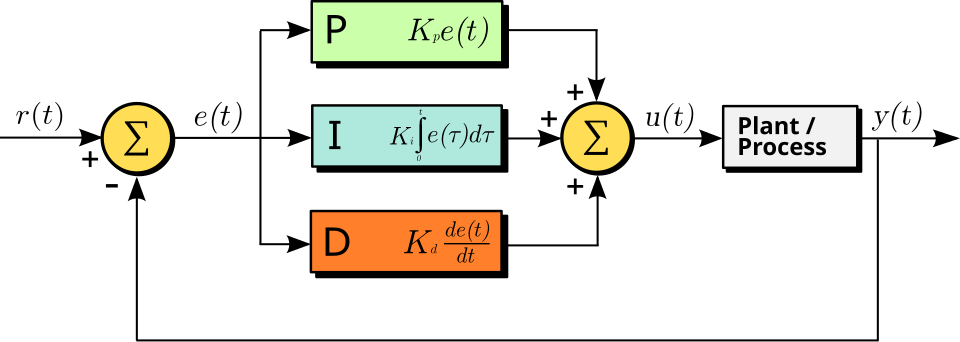
\includegraphics[width=0.8\columnwidth]{fig/PID_en.png}
	\caption{A visszacsatolást használó PID szabályzó blokkdiagramja. r(t) a kívánt folyamatváltozó (process variable, PV) or munkapont (setpoint, SP), és y(t) a PV mért értéke. (Wikipedia) \label{fig:PID_Controller}
	}
\end{figure}
\fi


\ifx\magyar\undefined
We considered that the neuron has a stable base state. On the one side, this resting state must be dynamically stabilized for little perturbations using as little energy as possible
(and to provide a mechanism when the cell grows, divides, or ages). On the other side, it must be able to restore the state after rough perturbations as quickly as possible, causing short-time transients (when restoring the
membrane's potential after issuing a spike).
In both the resting and transient states, the system attempts to return to its balanced state, though the mechanisms required differ. 

In its excited state, the system aims to provide an intense output that informs the downstream neurons.
This overshoot is initiated by a large number of voltage-gated ion channels (distinct from the non-gated ion channels used to maintain the resting potential) distributed in the neuron's membrane.
The overshoot current flows through those persistently open ion channels, which are concentrated in \gls{AIS} (which has about two orders of magnitude higher channel density than the wall).
The intense slow current produces a condenser-like behavior (capacitive current); the phenomena called "polarization" and "hyperpolarization" (not polarization; instead, a movement of completely separated charge in the surface layer of the electrolyte) of the membrane provide the necessary positive and negative error signals for the controller in the transient state by moving the actual potential value of the membrane above and below the resting potential value. The potentials and the electrical field's magnitudes 
depend on the concentration and the geometry (the finite size of the membrane). The ions' chemical nature comes into play only if the polarizability can differ 
for different molecules.

\else

We considered that the neuron has a stable base state. On the one side, this resting state must be dynamically stabilized for little perturbations using as little energy as possible
(and to provide a mechanism when the cell grows, divides, or ages). On the other side, it must be able to restore the state after rough perturbations as quickly as possible, causing short-time transients (when restoring the
membrane's potential after issuing a spike).
In both the resting and transient states, the system attempts to return to its balanced state, though the mechanisms required differ. 

In its excited state, the system aims to provide an intense output that informs the downstream neurons.
This overshoot is initiated by a large number of voltage-gated ion channels (distinct from the non-gated ion channels used to maintain the resting potential) distributed in the neuron's membrane.
The overshoot current flows through those persistently open ion channels, which are concentrated in \gls{AIS} (which has about two orders of magnitude higher channel density than the wall).
The intense slow current produces a condenser-like behavior (capacitive current); the phenomena called "polarization" and "hyperpolarization" (not polarization; instead, a movement of completely separated charge in the surface layer of the electrolyte) of the membrane provide the necessary positive and negative error signals for the controller in the transient state by moving the actual potential value of the membrane above and below the resting potential value. The potentials and the electrical field's magnitudes 
depend on the concentration and the geometry (the finite size of the membrane). The ions' chemical nature comes into play only if the polarizability can differ 
for different molecules.
\fi

\ifx\magyar\undefined
\subsection[Components]{Neuronal components \label{sec:AbstractComponents}}

\else

\subsection[Komponensek]{Neuron komponensek \label{sec:AbstractComponents}}
\fi

\ifx\magyar\undefined
\subsubsection[Ion channel]{Ion channel\label{sec:AbstractIonChannel}}

\else

\subsubsection[Ioncsatorna]{Ioncsatorna\label{sec:AbstractIonChannel}}
\fi



\ifx\magyar\undefined
\subsubsection[Electrolyte layer]{Layer of life\label{sec:AbstractLayer}}

\else

\subsubsection[Elektrolitréteg]{Az élet rétege\label{sec:AbstractLayer}}
\fi


\ifx\magyar\undefined

Embedded in the wall of the membrane, a smaller amount of (controlled 
and uncontrolled) ion channels are scattered.
Between the membrane and the axon, there is an array of a large amount of uncontrolled ion channels (the Axon Initial Segment \gls{AIS}). 
The elastic wall of the membrane is covered with ion layers, and therefore, a potential difference is created there (the resting potential).
The membrane represents \textit{a confined space in which ions behave differently from in an infinite space}; furthermore, it significantly alters the properties of the few-nanometer-thick electrolyte layer near the membrane. In this layer, the concentration and potential change significantly with the distance from the membrane due to interactions between the membrane's ion layers and the electrolyte.
Ion packages (spikes) sent by other neurons can enter the internal volume through controlled inputs (synapse).

\else

Embedded in the wall of the membrane, a smaller amount of (controlled 
and uncontrolled) ion channels are scattered.
Between the membrane and the axon, there is an array of a large amount of uncontrolled ion channels (the Axon Initial Segment \gls{AIS}). 
The elastic wall of the membrane is covered with ion layers, and therefore, a potential difference is created there (the resting potential).
The membrane represents \textit{a confined space in which ions behave differently from in an infinite space}; furthermore, it significantly alters the properties of the few-nanometer-thick electrolyte layer near the membrane. In this layer, the concentration and potential change significantly with the distance from the membrane due to interactions between the membrane's ion layers and the electrolyte.
Ion packages (spikes) sent by other neurons can enter the internal volume through controlled inputs (synapse).

\fi

%\ifx\magyar\undefined
%
%\section[Computing]{Computing\label{sec:Single-Computing}}
%
%\else
%
%
%\section[Computing]{Computing\label{sec:Single-Computing}}
%\fi
%
%
%\ifx\magyar\undefined
%
%
%We accept the truism that "The brain computes!"~\cite{KochBiophysics:1999} and elaborate in Chapter~\ref{ch:Computing}
%how neuronal computing can be interpreted in terms of 
%the general computing theory.
%Here we define the terms of abstract neuronal operation
%we use there and below when discussing the physical operation of the neuron.
%
%\else
%
%
%We accept the truism that "The brain computes!"~\cite{KochBiophysics:1999} and elaborate in Chapter~\ref{ch:Computing}
%how neuronal computing can be interpreted in terms of 
%the general computing theory.
%Here we define the terms of abstract neuronal operation
%we use there and below when discussing the physical operation of the neuron.
%\fi
%

